% Comment to allow building from within this file
%!TEX root = pyconuk2016.tex

\blankscreen{
  Substance Paridigm\textCR
  \textCR
}

\begin{frame}{}

    \tikzstyle{primary} = [
        rectangle, rounded corners, line width=0.4mm, draw=blue,
        minimum height=2cm, minimum width=3cm
    ]
    \tikzstyle{substance} = [
        rectangle, rounded corners, line width=0.4mm, draw=blue,
        top color=white, bottom color=blue!20,
        minimum height=2cm, minimum width=3cm
    ]
    \tikzstyle{attribute} = [
        rectangle, rounded corners, line width=0.4mm, draw=red,
        minimum width=2cm, fill=white, opacity=1
    ]
    \tikzstyle{hidden} = [
        rectangle, rounded corners,
        % line width=0.4mm, draw=green,
        minimum height=3cm, minimum width=6cm
    ]
    \tikzstyle{real} = [rectangle]
    \tikzstyle{line} = [line width=0.5mm]

    \begin{center}
        \resizebox{10cm}{!}{
            \begin{tikzpicture}
                \node[hidden](car) at (0, 9) {};
                    \node[hidden](mx5) at (-3, 6){};
                        \node[hidden](my_mx5) at (-3, 3){};
                            \node[hidden](real_mx5) at (-3, 0){};

                    \node[hidden](mondeo) at (3, 6){};
                        \node[hidden](my_mondeo) at (3, 3){};
                            \node[hidden](real_mondeo) at (3, 0){};

                \node[hidden](dwelling) at (9, 9){};
                    \node[hidden](house) at (9, 6){};
                        \node[hidden](my_house) at (9, 3){};
                            \node[hidden](real_house) at (9, 0){};


                \node<1->(1)[real] at (real_mx5){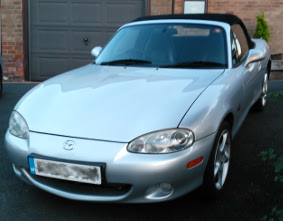
\includegraphics[width=3cm]{images/mx5}};

                \node<2->(2)[real] at (real_mondeo){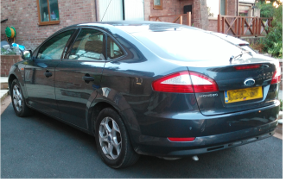
\includegraphics[width=3cm]{images/mondeo}};

                \node<3->(3)[real] at (real_house){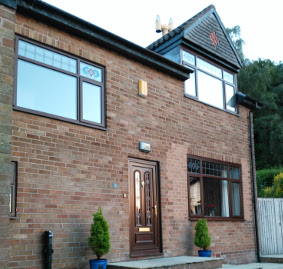
\includegraphics[width=3cm]{images/house}};

                \node<4->(4) at (my_mx5)[primary]{};
                \draw<4->(1.north)--(4.south);

                \node<5->(5) at (my_mondeo)[primary]{};
                \draw<5->(2.north) -- (5.south);

                \node<6->(6) at (my_house)[primary]{};
                \draw<6->(3.north) -- (6.south);

                \node<7->(silver)[attribute] at (4.east){Silver};
                \node<7->(abc123)[attribute, anchor=north west] at (silver.south west){ABC 123};

                \node<8->(grey)[attribute] at (5.east){Grey};
                \node<8->(xyz789)[attribute, anchor=north west] at (grey.south west){XYZ 789};

                \node<9->(detached)[attribute] at (6.east){Detached};
                \node<9->(1963)[attribute, anchor=north west] at (detached.south west){1963};

                \node<10->(7) at (mx5)[substance]{Mazda MX5};
                \draw<10->(4.north) -- (7.south);

                \node<11->(8) at (mondeo)[substance]{Ford Mondeo};
                \draw<11->(5.north) -- (8.south);

                \node<12->(9) at (house)[substance]{House};
                \draw<12->(6.north) -- (9.south);

                \node<13->(10) at (car)[substance]{Car};
                \draw<13->(7.north) -- (10.south);
                \draw<13->(8.north) -- (10.south);

                \node<14->(11) at (dwelling)[substance]{Dwelling};
                \draw<14->(9.north) -- (11.south);

            \end{tikzpicture}
        }
    \end{center}

\end{frame}
